\documentclass[lightblue, notheorems, xcolor=dvipsnames]{beamer}
%\usepackage{beamerthemeshadow}
\usetheme{Madrid}
\setbeamercolor{author in head/foot}{bg=structure.fg, fg=white} % Hintergrundfarbe wie structure.fg und Textfarbe weiß

\setbeamertemplate{footline}{%
	\hbox{%
		\begin{beamercolorbox}[wd=\paperwidth,ht=2.25ex,dp=1ex,center]{author in head/foot}%
			\insertframenumber/\inserttotalframenumber
		\end{beamercolorbox}%
	}%
}

\usepackage[english]{babel}
\usepackage[utf8]{inputenc}
\usepackage[T1]{fontenc}
\usepackage{amsmath, amssymb, amsthm, amsfonts} %einige hilfreiche Mathe-Pakete
\setbeamertemplate{theorems}[ams style]
\usepackage{tabularx, multirow} %fuer Tabellen
\usepackage{graphicx, tikz} %Grafiken
\usepackage{setspace} %Paket f\"ur das Formatieren von Quellen unten auf einer Folie
\newcommand{\diff}{\mathop{}\!\mathrm{d}}
\usepackage[T1]{fontenc}

% Algorithm
\usepackage[ruled,vlined]{algorithm2e}
\usepackage{algpseudocode}
\usepackage{algorithmicx}
\usepackage{arydshln} % gestrichelte Linie



% BIlder
\setbeamertemplate{caption}[numbered]
\usepackage{subcaption}
%\usepackage{subfig}
\usepackage{graphicx}
\usepackage{float}
%\usepackage{tikz}

\usepackage{comment}

% Ausblenden Navigation
\beamertemplatenavigationsymbolsempty

% definiere Enviroments
\theoremstyle{definition}
\newtheorem{defi}{Definition}[section]
\newtheorem{idea}{Idee}[section]
\theoremstyle{plain}
\newtheorem{theo}[defi]{Satz}
\newtheorem{coroll}[defi]{Korollar}%
\newtheorem{lem}[defi]{Lemma}%
\newtheorem{aim}[defi]{Ziel}
%\newtheorem*{proof}{Beweis}%[theorem]

% Zeichnen
\usepackage{tikz}
\usetikzlibrary{3d,arrows.meta,calc}

\theoremstyle{example}
\newtheorem{remark}[defi]{Bemerkung}%
\newtheorem{examp}[defi]{Beispiel}%
\newtheorem*{lsg}{Lösung}



\DeclareMathOperator*{\argmax}{argmax}


\iffalse
\expandafter\def\expandafter\insertshorttitle\expandafter{%
    \insertshorttitle\hfill%
    \insertframenumber\,/\,\inserttotalframenumber}
\fi



\SetKwRepeat{Do}{do}{while}%
\begin{document}
   %\maketitle  %erstellt Titelseite mit oben stehenden Informationen
  % optional: mit 
  \author{Bella My Phuong Quynh Duong, Christiane Helzel}
  \date{September 23, 2025} %Datum des Vortrags eintragen
  \institute{Heinrich-Heine University D\"usseldorf}
  \title{Three-Dimensional Modeling of Sedimentation in
  	Suspensions of Rod-Like Particles}
  
  \begin{frame}
  	\titlepage
  	\begin{figure}[htpb]
  		\begin{center}
  			
\includegraphics[width=0.2\textwidth]{logo.png}
  		\end{center}
  	\end{figure}
  \end{frame}
\begin{frame}
   \frametitle{Table of Contents}
\tableofcontents %dieser Befehl erzeugt das Inhaltsverzeichnis
\end{frame}

\AtBeginSection[]
{
	\begin{frame}<beamer>
		\frametitle{Overview}
		\tableofcontents[currentsection]
	\end{frame}
}

\section{Motivation}
\begin{frame}
    Guazzelli et al examined a dilute suspension of rod-like particles influenced by gravity.
\begin{columns}
	\begin{column}{0.5\textwidth}
		\begin{itemize}
			\item In an initially homogeneous suspension, rod-like particles form clusters where they are denser.
			\item The clusters create downward flows balanced by upward flows.
			\item Particles in a cluster mostly align with gravity, occasionally flipping.
		\end{itemize}
	\end{column}
	\begin{column}{0.5\textwidth}
		\begin{figure}[H]
			\centering
			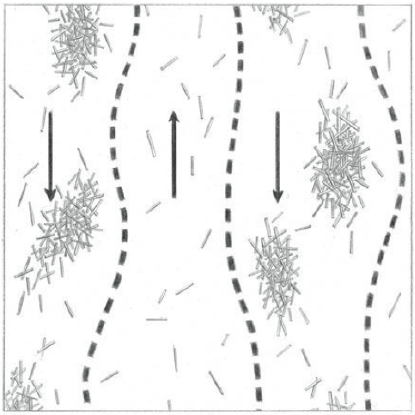
\includegraphics[scale=0.5]{Bilder/Bild_Particles}
		\end{figure}
	\end{column}
\end{columns}
\end{frame}

\begin{frame}{Mathematical Model for the Sedimentation of Rod-Like Particles}
	\scriptsize
\text{Coupling of a kinetic Smoluchowski equation with Navier-Stokes equation}
\begin{align*}
	\textcolor{blue}{\partial_t f}+ \textcolor{red}{\nabla_{\boldsymbol{x}} \cdot(\boldsymbol{u} f)} & +\textcolor{blue}{\nabla_{\boldsymbol{n}} \cdot\left(P_{\boldsymbol{n}^{\perp}} \nabla_{\boldsymbol{x}} \boldsymbol{u} \boldsymbol{n} f\right)}- \textcolor{red}{\nabla_{\boldsymbol{x}} \cdot\left((I+\boldsymbol{n} \otimes \boldsymbol{n}) e_3 f\right)} \\
	& =\textcolor{blue}{D_r \Delta_n f}+\gamma \nabla_{\boldsymbol{x}} \notag \cdot(I+\boldsymbol{n} \otimes \boldsymbol{n}) \nabla_{\boldsymbol{x}} f, \\
	\sigma & =\int_{S^{d-1}}(\text{d} \; \boldsymbol{n} \otimes \boldsymbol{n}-I) f d \boldsymbol{n},  \\
	\operatorname{Re}\left(\partial_t \boldsymbol{u}+\left(\boldsymbol{u} \cdot \nabla_{\boldsymbol{x}}\right) \boldsymbol{u}\right) & =\Delta_{\boldsymbol{x}} \boldsymbol{u}-\nabla_{\boldsymbol{x}} p+\delta \gamma \nabla_{\boldsymbol{x}} \cdot \sigma-\delta \int_{S^{d-1}} f d \boldsymbol{n} \, e_3, \\
	\nabla_{\boldsymbol{x}} \cdot \boldsymbol{u} & =0,
\end{align*}
where $f = f(\boldsymbol{x}, t, \boldsymbol{n}), \boldsymbol{x} \in \mathbb{R}^3 , \boldsymbol{n} \in  S^2$ is a density distribution function of particle orientation. $D_r, \gamma, \delta$ and $Re$ are non-dimensional parameters.
\begin{beamercolorbox}[sep=1em,wd=\linewidth,right]{}
	\tiny{Helzel $\&$ Tzavaras, 2017}
\end{beamercolorbox}
Here we consider the case $\gamma = 0$.
\end{frame}


\begin{frame}{Status of Project}
	\scriptsize
    \begin{block}{So far...}
    	\begin{itemize}
    		\item  Investigate hierarchy of moment equations for simplified model with \textcolor{cyan}{$f$ on $S^1$}
    		\begin{itemize}
    		\item <1->  Transform high dimensional scalar PDE (in space and orientation) into a lower dimensional system of moment equations (in
    		space)
    	   \item <2-> Investigate accuracy of moment closure system
    	    \end{itemize}
    	\end{itemize}
       	   Dahm, Helzel, MMS 2022, Dahm, Giesselmann, Helzel, JCP 2024
    \end{block}
	\begin{block}{Now}
		\begin{itemize}
			\item <3-> Derive and approximate hierarchies of moment equations for the coupled kinetic-fluid model with \textcolor{cyan}{$f$ on $S^2$}.
		\end{itemize}
	\end{block}
\end{frame}
%%%%%%%%%%%%%%%%%%%%%%%%%%%%%%%%%%%%%%%%%%%%%%%%%%%%%%
\begin{comment}
\begin{frame}{Spectral method}
	\scriptsize
	Consider the drift-diffusion equation
	\begin{align}
		\textcolor{blue}{\partial_t f}+ \textcolor{gray!80}{\nabla_{\boldsymbol{x}} \cdot(\boldsymbol{u} f)} & +\textcolor{blue}{\nabla_{\boldsymbol{n}} \cdot\left(P_{\boldsymbol{n}^{\perp}} \nabla_{\boldsymbol{x}} \boldsymbol{u} \boldsymbol{n} f\right)}-\textcolor{gray!80}{\nabla_{\boldsymbol{x}} \cdot\left((I+\boldsymbol{n} \otimes \boldsymbol{n}) e_3 f\right)} \notag \\
		& = \textcolor{blue}{D_r \Delta_n f}+\textcolor{gray!80}{\gamma \nabla_{\boldsymbol{x}} \cdot(I+\boldsymbol{n} \otimes \boldsymbol{n}) \nabla_{\boldsymbol{x}} f} \label{SmochEq_kurz}
	\end{align}
	with externally imposed velocity gradient $\nabla_x. \boldsymbol{u}_{\mathrm{ext}}$\\
	\vspace{12pt}
	\pause
	In spherical coordinates
	\begin{align}
		\underbrace{\sin \theta \partial_t f}_{[1]} + \underbrace{\partial_\phi\left(a(\phi, \theta) f\right)+\partial_\theta\left(b(\phi, \theta) f\right)}_{[2]} = \underbrace{D_r \left(\partial_\phi\left(\frac{1}{\sin \theta} \partial_\phi f\right)+\partial_\theta\left(\sin \theta \partial_\theta f\right)\right)}_{[3]}, \label{Smoch_S2}
	\end{align}	
	with $\phi \in [0, 2 \pi]$ and $\theta \in [0, \pi]$.\\
	\vspace{12pt}
	\pause
  Ansatz for our \textcolor{cyan}{spectral method}
\begin{align}
	f(x,t,\phi, \theta) \approx f_0(x,t) \cdot P_0^0 + \sum_{n=1}^{N} \sum_{k=-2n}^{2n} c^k_{2n}(x,t) \cdot P^k_{2n}(\phi, \theta), \label{ansatz}
\end{align}
where $P^k_{2n}(\phi, \theta)$ are harmonic polynomial basis functions.  %, i.e. are eigenfunctions of Laplace Beltrami operator.
\end{frame}

\begin{frame}{Example}
	\scriptsize
	For $N=1$ we obtain
	\begin{equation}
		\left(\begin{array}{c}
			f_0(t) \\
			c_2^{-2}(t) \\
			c_2^{-1}(t) \\
			c_2^0(t) \\
			c_2^1(t) \\
			c_2^2(t)
		\end{array}\right)^{\prime} - A \cdot
		\left(\begin{array}{c}
			f_0(t) \\
			c_2^{-2}(t) \\
			c_2^{-1}(t) \\
			c_2^0(t) \\
			c_2^1(t) \\
			c_2^2(t)
		\end{array}\right) = -6 D_r \cdot
		\left(\begin{array}{c}
			0 \\
			c^{-2}_2(t) \\
			c_2^{-1}(t) \\
			c_2^0(t) \\
			c_2^1(t) \\
			c_2^2(t)
		\end{array}\right),
	\end{equation}
\end{frame}

\begin{frame}
	where the matrix $A$ has the form \\
	\vspace{8pt}
	\begin{multline*}
		\resizebox{\textwidth}{!}{%
			\(
			\begin{pmatrix}
				\vspace{12pt}
				0 & 0 & 0 & 0 & 0 & 0 \\
				\vspace{12pt}
				\frac{1}{5}\sqrt{15}(u_x-v_y) & \frac{1}{7}(u_x+v_y-2w_z) & \frac{1}{7}(-5u_z+2w_x) & \frac{1}{7}\sqrt{3}(-u_x+v_y) & \frac{1}{7}(5v_z-2w_y) &  (u_y -v_x) \\
				\vspace{12pt}
				\frac{1}{5}\sqrt{15}(-u_z-w_x) & \frac{1}{7}(2u_z-5w_x) & \frac{1}{7}(u_x-2v_y+w_z) & \frac{1}{7}\sqrt{3}(-4u_z+3w_x) & \frac{1}{7}(5u_y-2v_x) &  \frac{1}{7} \left(2v_z-5w_y\right) \\
				\vspace{12pt}
				\frac{1}{5}\sqrt{5}(-u_x-v_y+2w_z) & \frac{1}{7}\sqrt{3}(-u_x+v_y) & \frac{1}{7}\sqrt{3}(3u_z-4w_x) & \frac{1}{7}(-u_x-v_y+2w_z) & \frac{1}{7}\sqrt{3}(-3v_z-4w_y) & \frac{1}{7} \sqrt{3}\left(-u_y-v_x\right) \\
				\vspace{12pt}
				\frac{1}{5}\sqrt{15}(-v_z-w_y) & \frac{1}{7}(-2v_z+5w_y) & \frac{1}{7}(-2u_y+5v_x) & \frac{1}{7}\sqrt{3}(-4v_z+3w_y) & \frac{1}{7}(-2u_x+v_y+w_z) &  \frac{1}{7} \left(2u_z-5w_x\right)\\
				\vspace{12pt}
				\frac{1}{5}\sqrt{15}(u_y+v_x) & (-u_y+v_x) & \frac{1}{7}(-5v_z+2w_y) & \frac{1}{7}\sqrt{3}(-u_y-v_x) & \frac{1}{7}(-5u_z+2w_x) & \frac{1}{7} \left(u_x+v_y-2w_z\right)
			\end{pmatrix}
			\).
		}
	\end{multline*}
\end{frame}
\end{comment}



\section{Hierarchy of Moment Equations for Shear Flow}
\begin{frame}{Ansatz for Derivation of Moment Equations}
	\scriptsize
    Consider approximation of the form
	\begin{align}
		\textcolor{cyan}{f(\textbf{x}, t, \phi, \theta) \approx f^N(\textbf{x},t,\phi,\theta) :=  \sum_{n=0}^{N} \sum_{i=-2n}^{2n} c^i_{2n}(\textbf{x},t) \cdot P^i_{2n}(\phi, \theta)}, \label{spectralmethod}
	\end{align}
	where $P^i_{2n}(\phi, \theta)$, $n = 0, \ldots, N$, $i = -2n, \ldots, 2n$
	\begin{itemize}
		\item are harmonic polynomial basis functions, i.e., the eigenfunctions of the Laplace-Beltrami operator with the eigenvalue $-2n(2n+1)$
		\pause
		\item form an orthonormal basis, wrt. the $L_2$-inner product on the sphere
		\begin{align*}
			(g,h)_{S^2} := \int_{0}^{2\pi} \int_{0}^{\pi} g(\phi, \theta) h(\phi, \theta) \cdot \sin(\theta) d\theta d\phi,
		\end{align*}
	\pause
	\item every square integrable function on $S^2$ can be expressed as a linear combination of spherical harmonics $f(\phi, \theta) = \sum^{\infty}_{n=0} \sum_{i=-n}^{n} c^i_{n} \cdot P^i_{n}(\phi, \theta)$.
	\end{itemize}
\end{frame}

\begin{frame}{Derivation of Moment Equations}
	\scriptsize
	We derive the moment equations by
	\begin{itemize}
		\item Insert ansatz $f^N =  \sum_{n=0}^{N} \sum_{i=-2n}^{2n} c^i_{2n}(x,t) \cdot P^i_{2n}(\phi, \theta)$ into kinetic equation
\begin{align*}
\sin\theta \partial_{t}f^N(x,t,\phi,\theta) + &  \textcolor{red}{\partial_x (\cos\phi \cos\theta \sin^2\theta f^N)} \\
	& 
	 =- \textcolor{blue}{\partial_\theta \left(w_x \sin^3 \theta \cos \phi f^N\right)} +\textcolor{blue}{D_{r} \left( \partial_\phi \left(\frac{1}{\sin \theta} \partial_\phi f^N \right) + \partial_\theta (\sin \theta \partial_\theta f^N) \right)}
\end{align*}
		\item Multiply consecutively with all basis functions used in the ansatz and integrate the resulting equations over the sphere
	\end{itemize}
\pause
The system of moment equations has the general form
\begin{align}
	\partial_t Q + \textcolor{red}{A\partial_x Q} = \textcolor{blue}{D(w_x)Q}+ \textcolor{blue}{D_rE Q},
\end{align}
where $Q=(c^0_0(x,t), c^{-2}_2(x,t), \ldots, c^{2N}_{2N}(x,t))^T$ represents the vector of the moments and \\
\vspace{2mm}
$A,D,E \in \mathbb{R}^{(N+1)(2N+1)x(N+1)(2N+1)}$.
\end{frame}

\begin{frame}{Derivation: A Closer Look}
\scriptsize
Consider 
\begin{align*}
	\textcolor{cyan}{\underbrace{\sin\theta \partial_{t}f^N(x,t,\phi,\theta)}_{[1]}} + &  \underbrace{\partial_x (\cos\phi \cos\theta \sin^2\theta f^N)}_{[2]} \\
	& 
	= -\partial_\theta \left(w_x \sin^3 \theta \cos \phi f^N\right) + D_{r} \left(\partial_\phi \left(\frac{1}{\sin \theta} \partial_\phi f^N \right) + \partial_\theta (\sin \theta \partial_\theta f^N) \right)
\end{align*}
\pause
For $k=0, \ldots, N$, $l=-2k, \ldots, 2k$ we obtain for term $[1]$
\begin{align*}
	&\int_{0}^{2\pi} \int_{0}^{\pi} \textcolor{cyan}{\sin\theta \partial_t \left(\sum_{n=0}^{N} \sum_{i=-2n}^{2n} c^i_{2n}(x,t) \cdot P^i_{2n}(\phi, \theta)\right)}P^l_{2k}(\phi, \theta) \\
	&= \sum_{n=0}^{N} \sum_{i=-2n}^{2n} \partial_t c^i_{2n}(x,t) \int_{0}^{2\pi} \int_{0}^{\pi} \sin\theta P^i_{2n}(\phi, \theta) P^l_{2k}(\phi, \theta) d\phi d\theta \\
	&=  \sum_{n=0}^{N} \sum_{i=-2n}^{2n} \partial_t c^i_{2n}(x,t) (P^i_{2n}(\phi, \theta) P^l_{2k}(\phi, \theta))_{S^2} =  \sum_{n=0}^{N} \sum_{i=-2n}^{2n} \partial_t c^i_{2n}(x,t) \cdot \delta_{n,k} \delta_{i,l} \\
	&= \partial_t c^l_{2k}(x,t)
\end{align*}
\pause
This corresponds to this term
$\textcolor{cyan}{\partial_t Q} + A\partial_x Q = D(w_x)Q+ D_rE Q$.
\end{frame}

\begin{frame}
	\scriptsize
Consider term [2]
\begin{align*}
	\underbrace{\sin\theta \partial_{t}f^N(x,t,\phi,\theta)}_{[1]} + &  \textcolor{cyan}{\underbrace{\partial_x (\cos\phi \cos\theta \sin^2\theta f^N)}_{[2]}} \\
	& 
	= -\partial_\theta \left(w_x \sin^3 \theta \cos \phi f^N\right) + D_{r} \left(\partial_\phi \left(\frac{1}{\sin \theta} \partial_\phi f^N \right) + \partial_\theta (\sin \theta \partial_\theta f^N) \right)
\end{align*}
\pause
This represents the term
$\partial_t Q + \textcolor{cyan}{A\partial_x Q} =  D(w_x)Q+ D_rEQ$ \\
\vspace{2mm}
For $N=1$ the matrix $A$ has the form
\begin{figure}[H]
		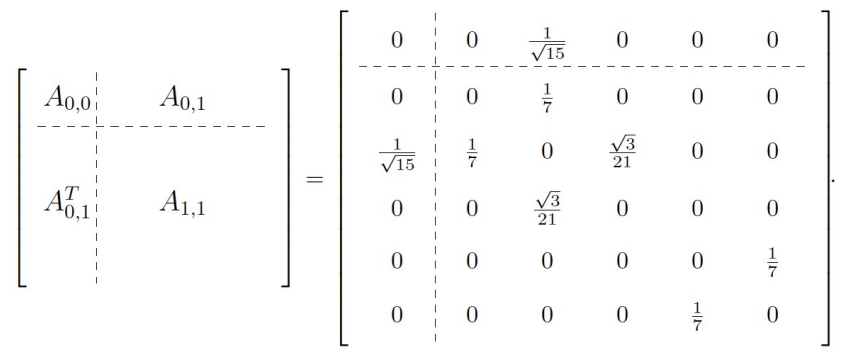
\includegraphics[scale=0.5]{Bilder/MatrixA}
\end{figure}
\end{frame}


\begin{comment}
	For $N=1$ the matrix $A$ has the form
	\begin{equation}
		\left[\begin{array}{c:c}
			A_{0,0} & A_{0,1} \\
			\hdashline A_{0,1}^T & A_{1,1}
		\end{array}\right]=\left[\begin{array}{c:ccccc}
			0 & 0 & \frac{1}{\sqrt{15}} & 0 & 0 & 0 \\
			\hdashline 0 & 0 & \frac{1}{7} & 0 & 0 & 0 \\
			\frac{1}{\sqrt{15}} & \frac{1}{7} & 0 & \frac{\sqrt{3}}{21} & 0 & 0 \\
			0 & 0 & \frac{\sqrt{3}}{21} & 0 & 0 & 0 \\
			0 & 0 & 0 & 0 & 0 & \frac{1}{7} \\
			0 & 0 & 0 & 0 & \frac{1}{7} & 0
		\end{array}\right] .
	\end{equation}
\end{comment}

%%%%%%%%%%%%%%%%%%%%%%%%%%%%%%%%%%%%%%%%%%%%%%%%%%%%%%%%%%%%%%%%%
%%%%%%%%%%%%%%%%% Struktur Matrix A N=2 machen %%%%%%%%%%%%%%%%%%
%%%%%%%%%%%%%%%%%%%%%%%%%%%%%%%%%%%%%%%%%%%%%%%%%%%%%%%%%%%%%%%%%


\begin{frame}
	\scriptsize
	For N = 2 the symmetric matrix A has the structure
\begin{figure}[H]
	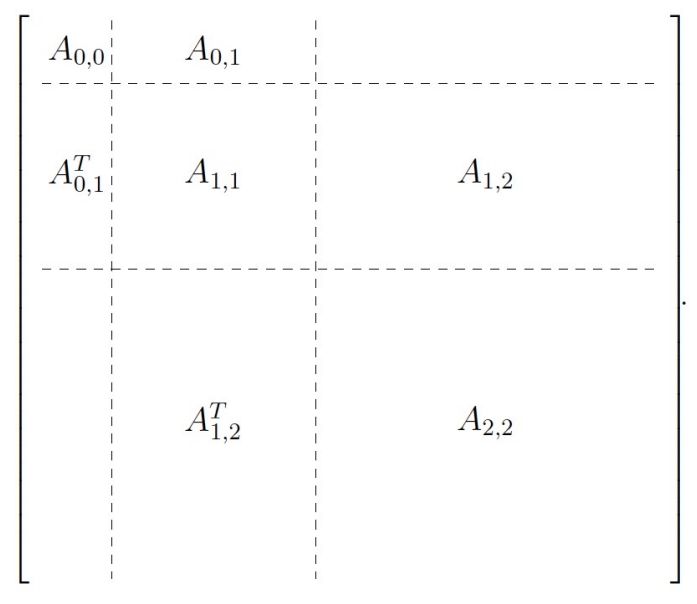
\includegraphics[scale=0.5]{Bilder/MatrixAN=2}
\end{figure}
\textcolor{cyan}{For any N the system of moment equations is hyperbolic.}
\end{frame}

\begin{frame}
		\scriptsize
Now consider the remaining terms:
	\begin{align*}
		\sin\theta \partial_{t}f^N(x,t,\phi,\theta) &+ \partial_x (\cos\phi \cos\theta \sin^2\theta f^N) \\
		&= \textcolor{cyan}{\underbrace{-\partial_\theta \left(w_x \sin^3 \theta \cos \phi f^N\right)}_{[3]} + \underbrace{D_{r} \left(\partial_\phi \left(\frac{1}{\sin \theta} \partial_\phi f^N \right) + \partial_\theta (\sin \theta \partial_\theta f^N) \right)}_{[4]}}.
	\end{align*}
\pause
\begin{itemize}
	\item Term $[4]$ corresponds to the Laplace-Beltrami operator,  resulting in $\textcolor{cyan}{D_r E Q}$, where the matrix $E$ is a diagonal matrix with the Laplace-Beltrami eigenvalues. 
	\pause
	\item Term $[3]$: We apply the same approach by inserting the ansatz for $f$ and projecting onto the polynomials, resulting in $\textcolor{cyan}{D(w_x)Q}$.
\end{itemize}
\vspace{5mm}
The system of moment equations:
$\partial_t Q + A\partial_x Q =  D(w_x)Q+ D_rEQ$. 
\end{frame}

\begin{comment}
\begin{frame}{Hierarchy of Moment Equations for Shear Flow}
\scriptsize
For $N=1$ we obtain 
\begin{equation}
	\begin{aligned}
		&\partial_t Q + \textcolor{red}{
			\begin{pmatrix}
				0 & 0 & \frac{\sqrt{15}}{15} & 0 & 0 & 0 \\
				0 & 0 & \frac{1}{7} & 0 & 0 & 0 \\
				\frac{\sqrt{15}}{15} & \frac{1}{7} & 0 & \frac{\sqrt{3}}{21} & 0 & 0 \\
				0 & 0 & \frac{\sqrt{3}}{21} & 0 & 0 & 0 \\
				0 & 0 & 0 & 0 & 0 & \frac{1}{7} \\
				0 & 0 & 0 & 0 & \frac{1}{7} & 0
		\end{pmatrix} \cdot \partial_x Q} \\
		&= \textcolor{blue}{
			\begin{pmatrix}
				0 & 0 & 0 & 0 & 0 & 0 \\
				0 & -6D_r & \frac{2}{7}w_x & 0 & 0 & 0 \\
				-\frac{\sqrt{15}}{5}w_x & -\frac{5}{7}w_x & -6D_r & \frac{3\sqrt{3}}{7}w_x & 0 & 0 \\
				0 & 0 & -\frac{4\sqrt{3}}{7}w_x & -6D_r & 0 & 0 \\
				0 & 0 & 0 & 0 & -6D_r & -\frac{5}{7} w_x \\
				0 & 0 & 0 & 0 & \frac{2}{7}w_x & -6D_r
			\end{pmatrix} Q }.
	\end{aligned}
\end{equation}
\end{frame}
\end{comment}




\section{Wave Propagation Algorithm}

\begin{frame}{Approximation of Coupled Shear Flow Problem}
	\scriptsize
	Consider
	\begin{equation}
		\begin{split}
			&\partial_t Q(x,t) + A\partial_x Q(x,t) =  D(w_x)Q(x,t)+ D_rEQ(x,t) \\
			&\partial_{t}w = \partial_{xx}w + \delta(\bar{\rho}-2\sqrt{\pi} c^0_0(x,t)).
		\end{split}
		\label{coupledsys_1d}
	\end{equation}
	\begin{table}[h]
		\centering
		\renewcommand{\arraystretch}{1.3}
		\scalebox{0.95}{
			\begin{tabular}{|c|l|}
				\hline
				1. & $\frac{1}{2} \Delta t$ step on $\partial_t Q(x, t) = (D(w_x(x,t_n))+ D_rE)Q(x,t)$ \\
				\hline
				2. & $\frac{1}{4} \Delta t$ step on $\partial_t w(x, t) = \delta(\bar{\rho} - 2\sqrt{\pi} c^0_0(x,t))$ \\
				3. & $\frac{1}{2} \Delta t$ step on $\partial_t w(x, t) = \partial_{xx} w(x, t)$ \\
				4. & $\frac{1}{4} \Delta t$ step on $\partial_t w(x, t) = \delta(\bar{\rho} -2\sqrt{\pi} c^0_0(x,t))$ \\
				\hline
				5. & $\Delta t$ step on $\partial_t Q(x, t) + A \partial_x Q(x, t) = 0$ \\
				\hline
				6. & $\frac{1}{4} \Delta t$ step on $\partial_t w(x, t) = \delta(\bar{\rho} - 2\sqrt{\pi} c^0_0(x,t))$ \\
				7. & $\frac{1}{2} \Delta t$ step on $\partial_t w(x, t) = \partial_{xx} w(x, t)$ \\
				8. & $\frac{1}{4} \Delta t$ step on $\partial_t w(x, t) = \delta(\bar{\rho} -2\sqrt{\pi} c^0_0(x,t))$ \\
				\hline
				9. & $\frac{1}{2} \Delta t$ step on $\partial_t Q(x, t) = (D(w_x(x,t_{n+1}))+ D_rE)Q(x,t)$ \\
				\hline
			\end{tabular}
		}
		\caption{Splitting algorithm for solving the coupled shear flow problem (Dahm et al.)}
	\end{table}
	We use an ODE solver for $1.+9.$, LeVeque’s high resolution wave propagation algorithm for $5.$ and finite difference methods for the evolution of $w$.
\end{frame}

%-------------------------------------------------------
%-------------------------------------------------------

\begin{frame}{1D Wave Propagation Algorithm (LeVeque et al.)}
	\scriptsize
	
	We consider the hyperbolic system
	\[
	q_t + f(q)_x = 0, \quad q \in \mathbb{R}^m
	\]
	
	\begin{itemize}
		\item Discretize the domain into cells $[x_{i-1/2}, x_{i+1/2}]$.
		\item At each interface $x_{i+1/2}$, solve the Riemann problem:
		\[
		q(x,0) = 
		\begin{cases} 
			q_i, & x < x_{i+1/2}, \\ 
			q_{i+1}, & x > x_{i+1/2}.
		\end{cases}
		\]
		\item Decompose the jump into waves along eigenvectors of $A = f'(q)$:
		\[
		q_{i+1} - q_i = \sum_{p=1}^m \alpha^p r^p, 
		\quad W^p = \alpha^p r^p, \; \text{travelling with } s^p.
		\]
		\item Define fluctuations:
		\[
		\mathcal{A}^+ \Delta q_{i-1/2} = \sum_{p: s^p>0} s^p W^p, \quad
		\mathcal{A}^- \Delta q_{i+1/2} = \sum_{p: s^p<0} s^p W^p
		\]
		\item Update cell averages:
		\[
		Q_i^{n+1} = Q_i^n - \frac{\Delta t}{\Delta x} 
		\Big( \mathcal{A}^+ \Delta q_{i-1/2} + \mathcal{A}^- \Delta q_{i+1/2} \Big)
		\]
	\end{itemize}
\end{frame}



%-------------------------------------------------------
%-------------------------------------------------------

\begin{frame}{Multidimensional Wave Propagation (2D and 3D)}
	\scriptsize
	\begin{columns}[c]
		
		%------------------ Linke Spalte: Theorie ------------------%
		\begin{column}{0.55\textwidth}
			\textbf{General system:}
			\[
			q_t + f(q)_x + g(q)_y + h(q)_z = 0
			\]
			
			\textbf{Key ideas:}
			\begin{itemize}
				\item \textbf{1D Riemann problems at cell interfaces:}  
				Solve along the normal direction of each cell interface.
				\item \textbf{Wave decomposition:}  
				Decompose jumps into waves \(W^p\) with speeds \(s^p\).
				\item \textbf{Fluctuations:}  
				\[
				\mathcal{A}^\pm \Delta q, \quad 
				\mathcal{B}^\pm \Delta q, \quad 
				\mathcal{C}^\pm \Delta q
				\]
				\item \textbf{Transverse propagation:}  
				\begin{itemize}
					\item 2D: Waves in \(x\)-direction generate waves in \(y\), and vice versa.
					\item 3D: Each wave generates transverse waves along in the other two directions.
				\end{itemize}
			\end{itemize}
		\end{column}
		
		%------------------ Rechte Spalte: Würfel ------------------%
		\begin{column}{0.45\textwidth}
			\centering
			    % 2D-Gitter
			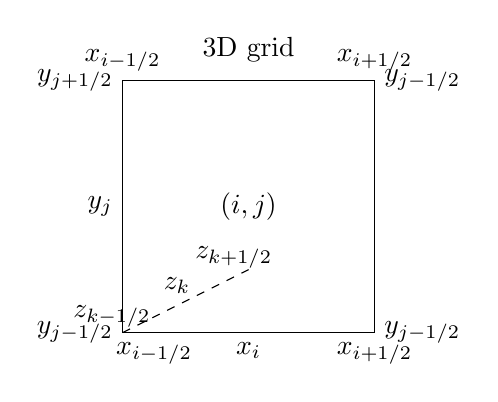
\begin{tikzpicture}[scale=0.8]
				% Titel
				\node at (2,4.5) {3D grid};
				% nur äußeres Quadrat
				\draw (0,0) rectangle (4,4);
				
				\node at (2,2) {$(i,j)$};
				
				% optionale äußere Beschriftungen
				\node[below] at (0.5,0) {$x_{i-1/2}$};
				\node[below] at (4,0) {$x_{i+1/2}$};
				\node[below] at (2,0) {$x_{i}$};
				\node[left]  at (0,4) {$y_{j+1/2}$};
				\node[left]  at (0,0.0) {$y_{j-1/2}$};
			    \node[left]  at (0,2) {$y_{j}$};
				\node[right]  at (4,0) {$y_{j-1/2}$};
				\node[right]  at (4,4) {$y_{j-1/2}$};
			    \node[above] at (4,4) {$x_{i+1/2}$};
				\node[above] at (0,4) {$x_{i-1/2}$};
				
				% z-Achse
                \draw[dashed] (0,0) -- (2,1);
                % Ursprung -> untere Zellkante
                \node[left] at (0.6,0.25) {$z_{k-1/2}$};
                % obere Zellkante
                \node[right] at (1,1.2) {$z_{k+1/2}$};
                % Zellzentrum
                \node[right] at (0.5,0.75) {$z_k$};
			\end{tikzpicture}
         % 1D-Gitter
       % \begin{tikzpicture}[scale=0.8]
 	   %  \foreach \i in {0,1,2} {\draw (\i,0) rectangle (\i+1,0.8);}
 	   %  \node at (1.5, 1) {1D grid};
 	    % \node at (0.5,0.4) {$i-1$};
 	    % \node at (1.5,0.4) {$i$};
 	   %  \node at (2.5,0.4) {$i+1$};
 	    % \node[below] at (1,0) {$x_{i-1/2}$};
 	   %  \node[below] at (2,0) {$x_{i+1/2}$};
       % \end{tikzpicture}
 
      %  \vspace{0.5cm} % Abstand zwischen den Grafiken
 	\end{column}
  	\end{columns}
\end{frame}


 \begin{comment}
        % 2D-Gitter
       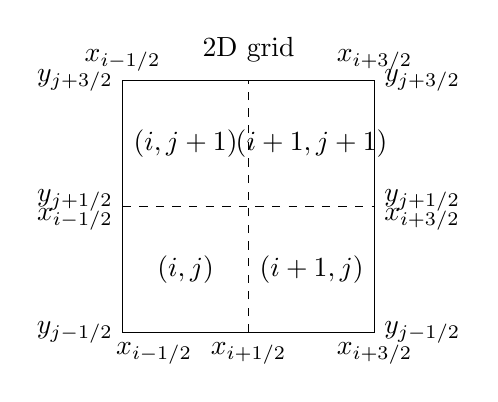
\begin{tikzpicture}[scale=0.8]
       	% Titel
       	\node at (2,4.5) {2D grid};
       % nur äußeres Quadrat
        \draw (0,0) rectangle (4,4);
      
       % Beschriftungen
        \node at (1,1) {$(i,j)$};
        \node at (3,1) {$(i+1,j)$};
        \node at (1,3) {$(i,j+1)$};
        \node at (3,3) {$(i+1,j+1)$};
      
       % Schnittlinien
        \draw[dashed] (2,0) -- (2,4);
        \draw[dashed] (0,2) -- (4,2);
       
       % optionale äußere Beschriftungen
       \node[below] at (0.5,0) {$x_{i-1/2}$};
       \node[below] at (2,0) {$x_{i+1/2}$};
       \node[below] at (4,0) {$x_{i+3/2}$};
       \node[left]  at (0,0.0) {$y_{j-1/2}$};
       \node[left]  at (0,2.1) {$y_{j+1/2}$};
       \node[left] at (0,1.8) {$x_{i-1/2}$};
       \node[left]  at (0,4) {$y_{j+3/2}$};
       \node[right]  at (4,0) {$y_{j-1/2}$};
       \node[right]  at (4,4) {$y_{j+3/2}$};
       \node[right] at (4,1.8) {$x_{i+3/2}$};
       \node[right]  at (4,2.1) {$y_{j+1/2}$};
 	   \node[above] at (0,4) {$x_{i-1/2}$};
 	   \node[above] at (4,4) {$x_{i+3/2}$};
      \end{tikzpicture}
\end{comment}

\begin{comment}
\begin{frame}{Multidimensional Wave Propagation (2D and 3D)}
	\scriptsize
	General system:
	\[
	q_t + f(q)_x + g(q)_y + h(q)_z = 0.
	\]
	
	\begin{itemize}
		\item At each cell face, solve a 1D Riemann problem in the normal direction.
		\item Decompose the jump into waves $W^p$ and corresponding speeds $s^p$.
		\item Compute fluctuations:
		\[
		\mathcal{A}^\pm \Delta q, \quad 
		\mathcal{B}^\pm \Delta q, \quad 
		\mathcal{C}^\pm \Delta q.
		\]
		\item Waves also propagate transversely:
		\begin{itemize}
			\item In 2D: a wave in $x-$direction can propagates in $y$-direction, and vice versa.
			\item In 3D: each wave generates transverse waves in the other two directions.
		\end{itemize}
	\end{itemize}
\end{frame}
\end{comment}

%-------------------------------------------------------
%-------------------------------------------------------

\begin{frame}{3D Transverse and Double Transverse Propagation}
	\scriptsize
	
    In 3D: every wave generates transverse and double–transverse contributions in the other directions

\vspace{0.5em} 
Examples of Transverse Interactions
		\begin{itemize}
			\item $x \to y$ (transverse) 
			\item $x \to z$ (transverse)
			\item $x \to y \to z$ (double transverse)
			\item $y \to x \to z$, etc.
		\end{itemize}

	\begin{block}{Update Scheme}
	\[
	\begin{aligned}
		Q_{i,j,k}^{n+1} &= Q_{i,j,k}^n
		- \frac{\Delta t}{\Delta x} \Big( \mathcal{A}^+ \Delta q_{i-1/2,j,k}
		+ \mathcal{A}^- \Delta q_{i+1/2,j,k} \Big) \\
		&\quad - \frac{\Delta t}{\Delta y} \Big( \mathcal{B}^+ \Delta q_{i,j-1/2,k}
		+ \mathcal{B}^- \Delta q_{i,j+1/2,k} \Big) \\
		&\quad - \frac{\Delta t}{\Delta z} \Big( \mathcal{C}^+ \Delta q_{i,j,k-1/2}
		+ \mathcal{C}^- \Delta q_{i,j,k+1/2} \Big).
	\end{aligned}
	\]
\end{block}
\end{frame}

%-------------------------------------------------------
%-------------------------------------------------------

\begin{comment}
\begin{frame}{Wave Propagation}
	\scriptsize
	The scheme can be specified by three integers $(m_1, m_2, m_3)$, which represent the following [LeVeque et. al]:
	\begin{align*}
		m_1 &= \left\{
		\begin{array}{ll}
			1, & \parbox[t]{0.6\textwidth}{The second order correction wave is not included,\\
				thus the method is formally first order accurate.} \\
			2, & \text{The correction wave is included.}
		\end{array}
		\right. \\
		m_2 &= \left\{
		\begin{array}{lll}
			0, & \text{No transverse propagation.} \\
			1, & \text{The propagation of the increment wave.} \\
			2, & \text{Transverse propagation of both increment and correction wave.}
		\end{array}
		\right. \\
		m_3 &= \left\{
		\begin{array}{lll}
			0, & \text{No double transverse propagation.} \\
			1, & \text{Double transverse propagation of the increment wave.} \\
			2, &  \parbox[t]{0.6\textwidth}{Double transverse propagation of both increment and \\
				correction wave.}
		\end{array}
		\right.
	\end{align*}
\end{frame}
\end{comment}
\section{Approximations of the Coupled Model}
\begin{frame}{Approximation of Coupled Shear Flow Problem}
	\scriptsize
	Consider
	\begin{equation}
		\begin{split}
			&\partial_t Q(x,t) + A\partial_x Q(x,t) =  D(w_x)Q(x,t)+ D_rEQ(x,t) \\
			&\partial_{t}w = \partial_{xx}w + \delta(\bar{\rho}-2\sqrt{\pi} c^0_0(x,t)).
		\end{split}
		\label{coupledsys_1d}
	\end{equation}
	\begin{table}[h]
		\centering
		\renewcommand{\arraystretch}{1.3}
		\scalebox{0.95}{
			\begin{tabular}{|c|l|}
				\hline
				1. & $\frac{1}{2} \Delta t$ step on $\partial_t Q(x, t) = (D(w_x(x,t_n))+ D_rE)Q(x,t)$ \\
				\hline
				2. & $\frac{1}{4} \Delta t$ step on $\partial_t w(x, t) = \delta(\bar{\rho} - 2\sqrt{\pi} c^0_0(x,t))$ \\
				3. & $\frac{1}{2} \Delta t$ step on $\partial_t w(x, t) = \partial_{xx} w(x, t)$ \\
				4. & $\frac{1}{4} \Delta t$ step on $\partial_t w(x, t) = \delta(\bar{\rho} -2\sqrt{\pi} c^0_0(x,t))$ \\
				\hline
				5. & $\Delta t$ step on $\partial_t Q(x, t) + A \partial_x Q(x, t) = 0$ \\
				\hline
				6. & $\frac{1}{4} \Delta t$ step on $\partial_t w(x, t) = \delta(\bar{\rho} - 2\sqrt{\pi} c^0_0(x,t))$ \\
				7. & $\frac{1}{2} \Delta t$ step on $\partial_t w(x, t) = \partial_{xx} w(x, t)$ \\
				8. & $\frac{1}{4} \Delta t$ step on $\partial_t w(x, t) = \delta(\bar{\rho} -2\sqrt{\pi} c^0_0(x,t))$ \\
				\hline
				9. & $\frac{1}{2} \Delta t$ step on $\partial_t Q(x, t) = (D(w_x(x,t_{n+1}))+ D_rE)Q(x,t)$ \\
				\hline
			\end{tabular}
		}
		\caption{Splitting algorithm for solving the coupled shear flow problem (Dahm et al.)}
	\end{table}
	We use an ODE solver for $1.+9.$, LeVeque’s high resolution wave propagation algorithm for $5.$ and finite difference methods for the evolution of $w$.
\end{frame}


%----------------------------------------------------------


\begin{frame}{Numerical Result for Shear Flow}
		\scriptsize
		Let 
		\begin{align*}
			c^0_0 (x,0) = (1+(1\cdot10^{-4} \cdot \eta(x)-5\cdot10^{-5}))/(2\sqrt{\pi}),
		\end{align*}
		where $\eta(x)$ is a random variable taking values in the interval $\pm \frac{1}{2}$.
		
		\begin{figure}
			\centering
			\begin{minipage}{0.46\textwidth}
				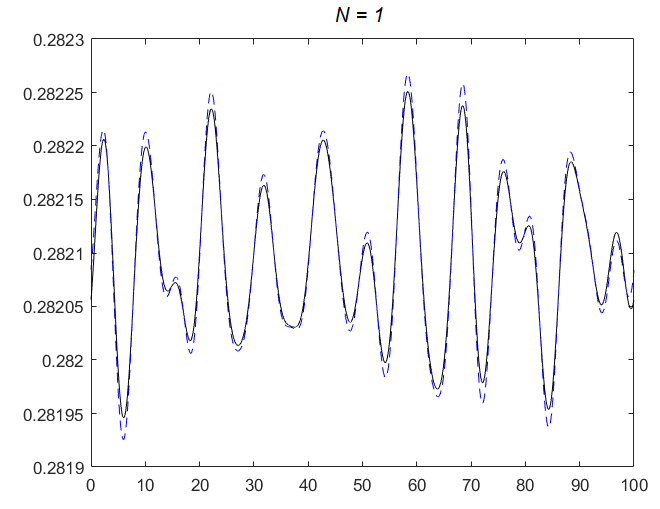
\includegraphics[width=\textwidth]{Bilder_wx/ClusterFormation/N=1vsN=6_Dr=0.05_mx=8192}
			\end{minipage}
			\hfill
			\begin{minipage}{0.46\textwidth}
				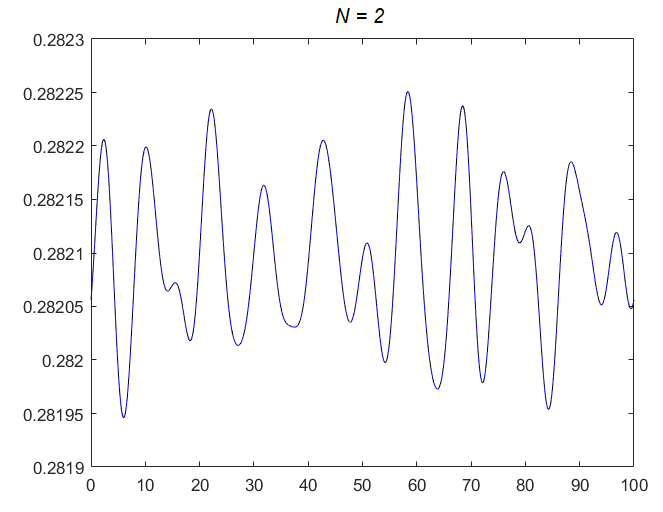
\includegraphics[width=\textwidth]{Bilder_wx/ClusterFormation/N=2vsN=6_Dr=0.05_mx=8192}
			\end{minipage}
			\caption{Approximation of the coupled problem for shear flow with $D_r =0.05$. The plot shows the density at time $t=30$ for $N = 1$ and $N = 2$ (blue line). A reference solution is calculated with $N = 6$ moment equations (black line).}
			\label{ClusterFormation}
		\end{figure}
		%The Figure (\ref{ClusterFormation}) shows that using $N = 1$ moment equations, compared to the reference solution with $N = 6$, already provides a good approximation of cluster formation. The numerical solution for $N=2$ aligns very well with the reference solution.
\end{frame}


%----------------------------------------------------------


\begin{frame}{Approximations of the Two-Dimensional Hyperbolic System}
		\scriptsize
		\begin{figure}[H]
			\centering
			\begin{minipage}{0.4\textwidth}
				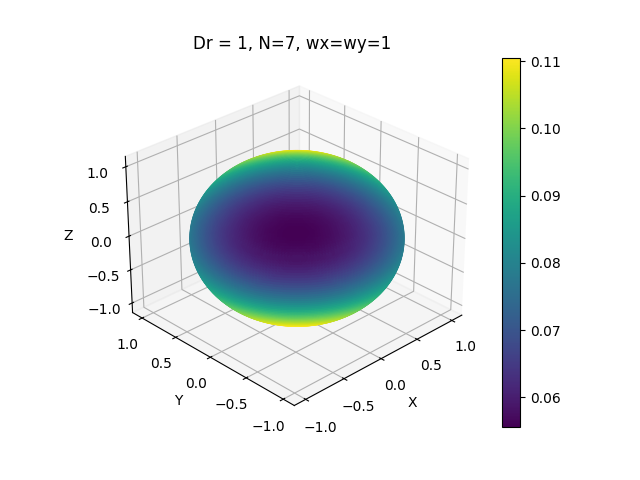
\includegraphics[scale=0.23]{Bilder_wxwy/Sol_onSphere_wx=1=wy_Dr=1_N=7}
			\end{minipage}
			\hfill 
			\begin{minipage}{0.4\textwidth}
				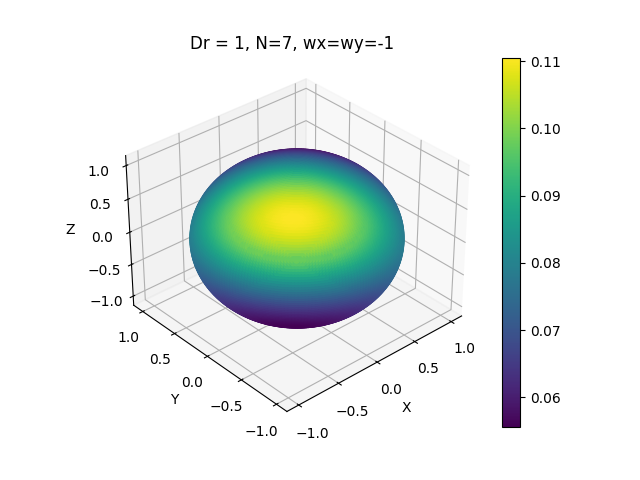
\includegraphics[scale=0.23]{Bilder_wxwy/Sol_onSphere_wx=-1=wy_Dr=1_N=7}
			\end{minipage}
			\caption{Numerical solution of the drift-diffusion term for fixed $w_x$ and $w_y$.}
		\end{figure}
		\begin{figure}[H]
			\centering
			\begin{minipage}{0.4\textwidth}
				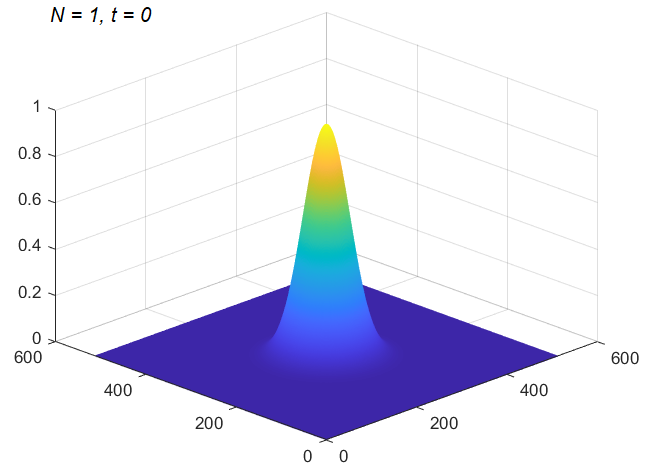
\includegraphics[scale=0.23]{Bilder_wxwy/t=0_wxwy=1_wxwy=-1}
			\end{minipage}
			\hfill 
			\begin{minipage}{0.4\textwidth}
				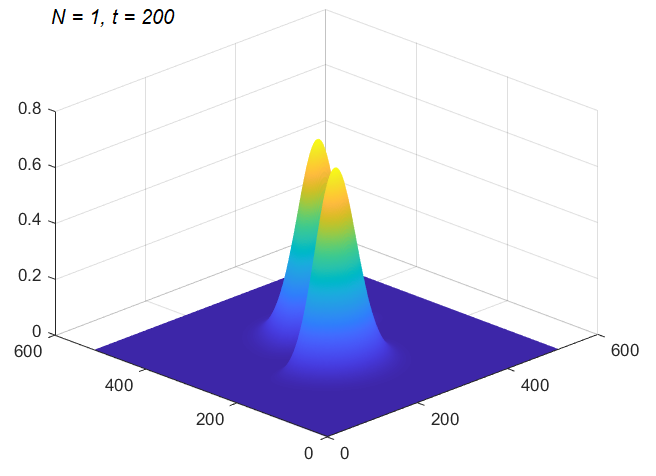
\includegraphics[scale=0.23]{Bilder_wxwy/t=200_wxwy=1_wxwy=-1}
			\end{minipage}
			\caption{Numerical results for $c^0_0$ at different times using $D_r=1$ and $w_x=w_y=1$ for $x<50$ and $w_x=w_y=-1$ otherwise. A cluster with higher particle density splits into two, each moving in opposite directions.}
		\end{figure}
\end{frame}

\begin{frame}{Conclusion}
	Inhalt...
\end{frame}

\begin{comment}
\begin{frame}{Appendix}
		\begin{table}[H]
			\scriptsize
			\begin{tabular}{|c|c|}
				\hline
				0th order	& 2nd order \\
				\hline
				& $P^{-2}_2 = \sqrt{\frac{15}{16\pi}}\sin^2(\theta)\cos(2\phi)$ \\
				& $P^{-1}_2 = \sqrt{\frac{15}{4\pi}}\sin(\theta)\cos(\theta)\cos(\phi)$ \\
				$P^0_0 = \sqrt{\frac{1}{4\pi}} \cdot 1$	& $P^0_2 = \sqrt{\frac{45}{16\pi}}\cos^2(\theta) - \frac{1}{3}$  \\
				&  $P^1_2 = \sqrt{\frac{15}{4\pi}}\sin(\theta)\cos(\theta)\sin(\phi)$\\
				&  $P^2_2 = \sqrt{\frac{15}{16\pi}}\sin^2(\theta)\sin(2\phi)$\\
				\hline
			\end{tabular}
			\caption{Normalized harmonic polynomial basis functions}
		\end{table}
\end{frame}
\end{comment}


\begin{comment}
\begin{frame}
	\centering
	Thank you for listening!
\end{frame}
\end{comment}

\AtBeginSection[]
%{
% \begin{frame}<beamer>
% \frametitle{Table of Contents}
% \tableofcontents[currentsection]
% \end{frame}
%}



%Ende
%\begin{frame}{Ende}
%	\centering
%	Thank you for listening!
%\end{frame}

\begin{comment}
\begin{frame}[allowframebreaks]
  \frametitle{Literatur}
  \nocite{*} %es werden auch Quellen aufgefuehrt, die nicht in den Folien zitiert sind.
  \bibliography{Bibliothek}
  \bibliographystyle{abbrv}
\end{frame}
\end{comment}

\end{document}